%& /home/jason/.config/TikzEdtWForms/TikzEdtWForms/1.0.0.0/temp_header
\begin{document}
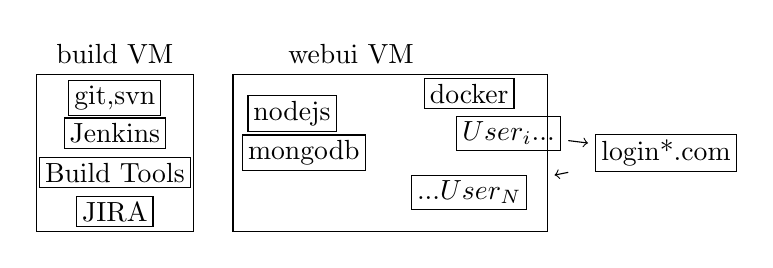
\begin{tikzpicture}

\tikzstyle{mynodestyle} = [draw,outer sep=0,inner sep=1,minimum size=10]

\draw  (0.0,-0.0) rectangle (2.0,-2.0); \node at (1.0,0.25) {build VM};
\draw  (2.5,-0.0) rectangle (6.5,-2.0); \node at (4.0,0.25) {webui VM};

\node [draw,outer sep=10,inner sep=2,minimum size=10] at (1.0,-0.3) {git,svn};

\node [draw,outer sep=10,inner sep=2,minimum size=10] at (1.0,-0.75) {Jenkins};
\node [draw,outer sep=10,inner sep=2,minimum size=10] at (1.0,-1.25) {Build Tools};
\node [draw,outer sep=10,inner sep=2,minimum size=10] at (1.0,-1.75) {JIRA};

\node [draw,outer sep=10,inner sep=2,minimum size=10] at (3.25,-0.5) {nodejs};
\node [draw,outer sep=10,inner sep=2,minimum size=10] at (3.4,-1.0) {mongodb};

\node [draw,outer sep=10,inner sep=2,minimum size=10] at (5.5,-0.25) {docker};

\node [draw,outer sep=10,inner sep=2,minimum size=10] (v2) at (6.0,-0.75) {$User_i$...};
\node [draw,outer sep=10,inner sep=2,minimum size=10] (v3) at (5.5,-1.5) {...$User_N$};

\node [draw,outer sep=10,inner sep=2,minimum size=10] (v1) at (8,-1) {login*.com};




\draw [->] (v1) edge (v2);
\draw [->] (v1) edge (v3);

\usetikzlibrary{calc}
\pgftransformreset
\node[inner sep=0pt,outer sep=0pt,minimum size=0pt,line width=0pt,text width=0pt,text height=0pt] at (current bounding box) {};
%add border to avoid cropping by pdflibnet
\foreach \border in {0.1}
  \useasboundingbox (current bounding box.south west)+(-\border,-\border) rectangle (current bounding box.north east)+(\border,\border);
\newwrite\metadatafile
\immediate\openout\metadatafile=\jobname_BB.txt
\path
  let
    \p1=(current bounding box.south west),
    \p2=(current bounding box.north east)
  in
  node[inner sep=0pt,outer sep=0pt,minimum size=0pt,line width=0pt,text width=0pt,text height=0pt,draw=white] at (current bounding box) {
\immediate\write\metadatafile{\p1,\p2}
};
\immediate\closeout\metadatafile
\end{tikzpicture}

\end{document}
